\begin{figure}
\centering
\begin{subfigure}{.3\textwidth}
  \centering
  \[
    \zooLoc \iPointstoTwo \zooVal_2
  \]
  \scalebox{.8}{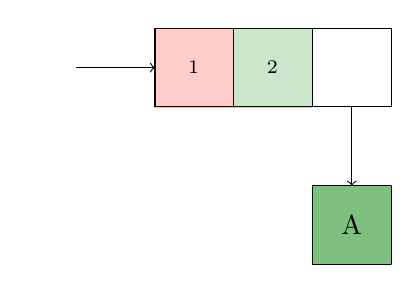
\begin{tikzpicture}[yscale=-1]
    \node at (0.5,0.5) {$\zooLoc$} ;
    \draw [->] (1,0.5) -- ++(1,0) ;
    \draw (2,0) grid ++(3,1) ;
    \draw [fill=red, opacity=0.2] (2,0) rectangle ++(1,1) ;
    \node at (2.5,0.5) {$\zooVal_1$} ;
    \draw [fill=Green, opacity=0.2] (3,0) rectangle ++(1,1) ;
    \node at (3.5,0.5) {$\zooVal_2$} ;
    \node at (4.5,0.5) {$\mcas$} ;
    \draw [->] (4.5,1) -- ++(0,1) ;
    \draw (4,2) grid ++(1,1) ;
    \draw [fill=Green, opacity=0.5] (4,2) rectangle ++(1,1) ;
    \node at (4.5,2.5) {A} ;
  \end{tikzpicture}}
  \caption{Successful MCAS}
  \label{fig:loc_representation_1}
  \end{subfigure}
\hfill
\begin{subfigure}{.3\textwidth}
  \centering
  \[
    \zooLoc \iPointstoTwo \zooVal_1
  \]
  \scalebox{.8}{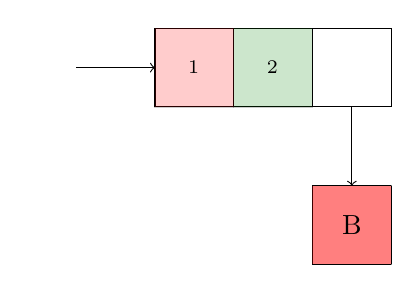
\begin{tikzpicture}[yscale=-1]
    \node at (0.5,0.5) {$\zooLoc$} ;
    \draw [->] (1,0.5) -- ++(1,0) ;
    \draw (2,0) grid ++(3,1) ;
    \draw [fill=red, opacity=0.2] (2,0) rectangle ++(1,1) ;
    \node at (2.5,0.5) {$\zooVal_1$} ;
    \draw [fill=Green, opacity=0.2] (3,0) rectangle ++(1,1) ;
    \node at (3.5,0.5) {$\zooVal_2$} ;
    \node at (4.5,0.5) {$\mcas$} ;
    \draw [->] (4.5,1) -- ++(0,1) ;
    \draw (4,2) grid ++(1,1) ;
    \draw [fill=red, opacity=0.5] (4,2) rectangle ++(1,1) ;
    \node at (4.5,2.5) {B} ;
  \end{tikzpicture}}
  \caption{Failed MCAS}
  \label{fig:loc_representation_2}
\end{subfigure}
\hfill
\begin{subfigure}{.38\textwidth}
  \centering
  \[
    \zooLoc \iPointstoTwo \zooVal_1
  \]
  \scalebox{.8}{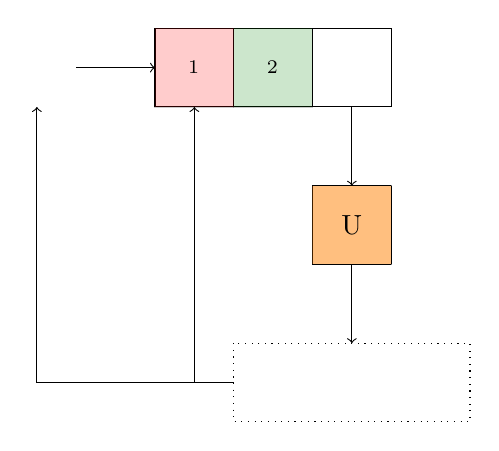
\begin{tikzpicture}[yscale=-1]
    \node at (0.5,0.5) {$\zooLoc$} ;
    \draw [->] (1,0.5) -- ++(1,0) ;
    \draw (2,0) grid ++(3,1) ;
    \draw [fill=red, opacity=0.2] (2,0) rectangle ++(1,1) ;
    \node at (2.5,0.5) {$\zooVal_1$} ;
    \draw [fill=Green, opacity=0.2] (3,0) rectangle ++(1,1) ;
    \node at (3.5,0.5) {$\zooVal_2$} ;
    \node at (4.5,0.5) {$\mcas$} ;
    \draw [->] (4.5,1) -- ++(0,1) ;
    \draw (4,2) grid ++(1,1) ;
    \draw [fill=orange, opacity=0.5] (4,2) rectangle ++(1,1) ;
    \node at (4.5,2.5) {U} ;
    \draw [->] (4.5,3) -- ++(0,1) ;
    \draw [dotted] (3,4) rectangle ++(3,1) ;
    \draw [->] (3,4.5) -| (0.5,1) ;
    \draw [->] (3,4.5) -| (2.5,1) ;
  \end{tikzpicture}}
  \caption{Undetermined MCAS}
  \label{fig:loc_representation_3}
\end{subfigure}
\caption{Representation of locations}
\label{fig:loc_representation}
\end{figure}
